% Unofficial UChicago CS Poster Template
% v1.1.0 released September 8, 2022
% https://github.com/k4rtik/uchicago-poster
% a fork of https://github.com/anishathalye/gemini

\documentclass[final,xcolor={dvipsnames,svgnames,table}]{beamer}

% ====================
% Packages
% ====================

\usepackage[T1]{fontenc}
\usepackage{lmodern}
\usepackage[size=custom,width=118.9,height=84.1,scale=1.0]{beamerposter}
\usetheme{gemini}
\usepackage{ragged2e}
\usecolortheme{insee}
\usepackage{graphicx}
\usepackage{booktabs}
\usepackage{doi}
\usepackage[numbers]{natbib}
\usepackage[patch=none]{microtype}
\usepackage{tikz}
\usepackage{pgfplots}
\pgfplotsset{compat=1.18}
\usepackage{anyfontsize}

\pdfstringdefDisableCommands{%
\def\translate#1{#1}%
}

% ====================
% Lengths
% ====================

% If you have N columns, choose \sepwidth and \colwidth such that
% (N+1)*\sepwidth + N*\colwidth = \paperwidth
\newlength{\sepwidth}
\newlength{\colwidth}
\setlength{\sepwidth}{0.025\paperwidth}
\setlength{\colwidth}{0.3\paperwidth}

\newcommand{\separatorcolumn}{\begin{column}{\sepwidth}\end{column}}

\definecolor{intersection}{RGB}{34, 177, 76}
\definecolor{primary}{RGB}{163, 73, 164}
\definecolor{second1}{RGB}{255, 201, 14}
\definecolor{second2}{RGB}{255, 127, 39}

% ====================
% Title
% ====================

\title{About releasing protected grid data on multiple levels}

\author{Clément Guillo \inst{1} \and Julien Jamme \inst{1}}

\institute[shortinst]{\inst{1} Insee (French National Statistical Institute)}

% ====================
% Footer (optional)
% ====================

\footercontent{
  \href{https://www.insee.fr}{https://www.insee.fr} \hfill
  NTTS Conference 2023, Brussels \hfill
  Contact us: \href{mailto:clement.guillo@insee.fr}{clement.guillo@insee.fr} or \href{mailto:julien.jamme@insee.fr}{julien.jamme@insee.fr}}
% (can be left out to remove footer)

% ====================
% Logo (optional)
% ====================

% use this to include logos on the left and/or right side of the header:
% \logoright{\includegraphics[height=7cm]{logo1.pdf}}
% \logoleft{\includegraphics[height=7cm]{logo2.pdf}}

% ====================
% Body
% ====================

\begin{document}
\addtobeamertemplate{headline}{}
{
    \begin{tikzpicture}[remember picture,overlay]
      \node [anchor=north west, inner sep=3cm] at ([xshift=0.0cm,yshift=2cm]current page.north west)
      {
\includegraphics[height=7.0cm]{logos/insee_logoanglaistransparent.png}}; % also try shield-white.eps
      %\node [anchor=north east, inner sep=3cm] at ([xshift=0.0cm,yshift=2.5cm]current page.north east)
      %{
\includegraphics[height=7.0cm]{logos/INSEE_1.1.png}};
    \end{tikzpicture}
}

\begin{frame}[fragile,t]
\begin{columns}[t]
\separatorcolumn

\begin{column}{\colwidth}
  \vspace{-1cm}
  \begin{block}{Context}

   The French national institute of statistics (Insee) is about to release Census data on two grids, measuring respectively 1km and 200m sideways. At the same time, these data are also available on administrative areas, such as municipalities. In this work, we focus only on the Metropolitan France, \textit{i.e.} without outermost regions.

   The release has to ensure the following \textbf{confidentiality rules}:

   \begin{itemize}
      \item \textbf{Threshold rule}: Original data in a square can not be released if less than 11 households live in it.
      \item \textbf{Sensitive attributes}: Users can not infer with more than 80\% confidence that \og all inhabitants in a given square are born abroad or have arrived from a foreign country \fg.
      \item \textbf{Exception}: the count of people in a square is not a confidential piece of information.
    \end{itemize}

   %The poster presents an \textit{\textbf{ongoing work}}.

  \end{block}

  \begin{backblock}{Confidentiality issues and objectives}

   \begin{itemize}
      \item \underline{\textbf{Disclosure by inter-level differentiation}}: The release of two (or more) levels of grid data has to be taken into account during the protection process.

      \begin{columns}[t]
      
        \begin{column}{0.4\colwidth}
                     
            \vspace{-1.5cm}
            
           \begin{figure}
             \centering
             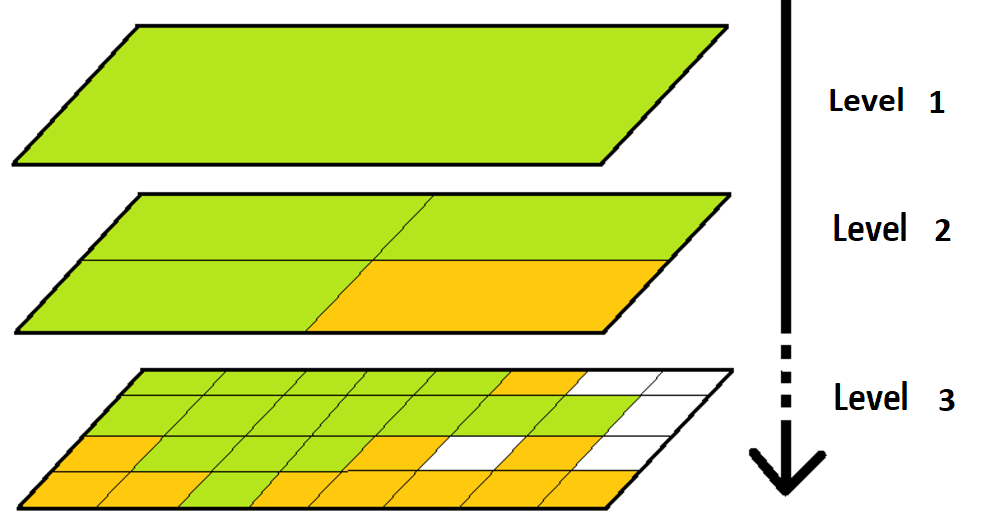
\includegraphics[scale=0.7]{Images/idea_multi_level.png}
          
             \vspace{-0.5cm}
                      
             \caption{Disclosure by inter-level diff.}
           \end{figure}

        \end{column}
          
        \separatorcolumn
          
        \begin{column}{0.4\colwidth}
            
            \vspace{1cm}

            \begin{itemize}
                \item 1km level: 375~159 non empty tiles - 52.6\% are below the threshold and 31~tiles are sensitive.
                \item 200m level: 2~224~377 non empty tiles - 78.1\% below the threshold and 232~tiles are sensitive.
            \end{itemize}
        \end{column}

      \end{columns}

           
      \item \underline{\textbf{Disclosure by overlapping differentiation}}: This issue comes from the concomitant release of the same information on grids and on administrative areas. These two kinds of zonings are not nested.
      \begin{columns}[t]
      
          \begin{column}{0.4\colwidth}
                     
            \vspace{-1.5cm}
                     
              \begin{figure}
                  \centering
                  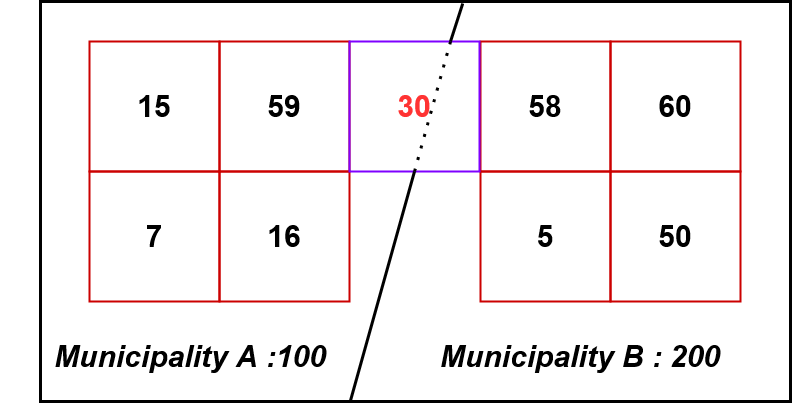
\includegraphics[scale=0.67]{Images/carreau_com.png}

                  \vspace{-0.5cm}
                  
                 \caption{Disclosure by non-nesting diff.}
                 
                  \label{fig:my_label}
            \end{figure}
          \end{column}
          
          \separatorcolumn
          
          \begin{column}{0.4\colwidth}
          
          \vspace{1cm}
          
          % In this simple example with only two municipalities, we can disclose a confidential information. Indeed, it's possible to know that only 3 households live in the intersection between the municipality A and the central purple square: 
          There are always two ways to make a differentiation:
              \begin{itemize}
                \item \textbf{Disclosure by internal differentiation}: $100 - (15+59+7+16) = 3$ 
                \item \textbf{Disclosure by external differentiation}: $(58+60+5+50+30) - 200 = 3$
            \end{itemize}
          \end{column}

      \end{columns}

    \end{itemize}
      % \item Other issues:
      % \begin{itemize}
      %     \item sensitive attributes to protect agaisnt inference, 
      %     \item disclose the original population count but perturbed ones for the population's attributes 
      % \end{itemize}

      \hrule 

      \vspace{0.25cm}
      
      \begin{columns}[t]
      
          \begin{column}{0.48\colwidth}
          
            \underline{\textbf{Other constraints}}
            \normalsize
            \begin{itemize}
              \item Inference disclosure risk of sensitive attributes
              \item Original population counts are released as they are, While other counts may be perturbed.
            \end{itemize}
              
          \end{column}
          
        \hfill
          
        \begin{column}{0.48\colwidth}
            
            \underline{\textbf{Additional objectives}}
            \normalsize          
            \begin{itemize}
              \item \textbf{Preserve additivity within squares}
              \item \textbf{Actual empty squares have to remain empty}
              \item \textbf{Preserve spatial structures}
            \end{itemize} 
            
        \end{column}

      \end{columns}
      
 

  \end{backblock}

  % \vspace{-1cm}
  \begin{block}{An alternative: the Cell Key Method}

    The Cell Key Method (CKM) is an efficient method designed to protect tabular data by adding noise into cells. As grids can be viewed as tables, the CKM was proposed as a relevant method to publish Census grid data (\cite{censusmeth}). 
    
    But, it shows some limitations in handling all our confidentiality issues and objectives:
    
    \begin{itemize}
        \item In adding a key to each individual to produce consistent tables, CKM can't at the same time release the original count of a cell while perturbing the counts of attributes.
        \item The CKM doesn't let us monitor how the spatial structures are perturbed.
        \item Despite the perturbation of squares by CKM, there are still differentiation issues with the municipality level. Indeed, some of these issues may concern big squares that have a high probability of being unperturbed.
    \end{itemize}

  \end{block}
% }

\end{column}

\separatorcolumn

\begin{column}{\colwidth}
  \vspace{-1cm}
  \begin{block}{1-Detect cells at risk of overlapping differentiation}

The detection of intersections between squares and municipalities at risk of differentiation relies on a method implemented in the \texttt{R} package called \texttt{diffman}. This method is based on a \textbf{graph modeling} in which two municipalities are connected if there is a square whose population is located in both of them. 

This representation allows to drastically limit the space of research of the differentiation problems and to extract quasi exhaustively the risky intersections in a reasonable time (\cite{costemalle2019}).

\begin{columns}
    \begin{column}{0.48\colwidth}
        \begin{figure}
            \centering
            \caption{Geographic representation}
            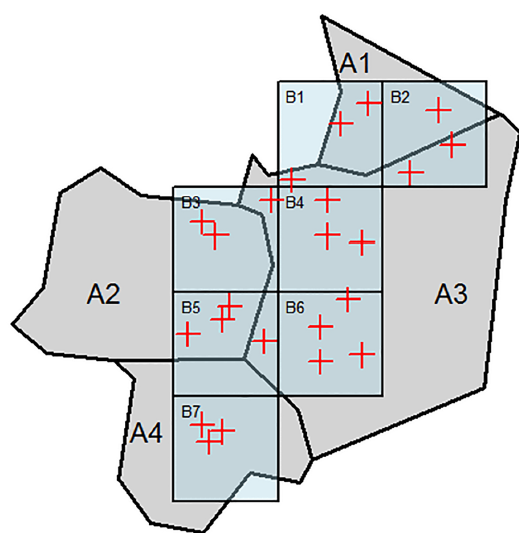
\includegraphics[scale=0.75]{Images/example_canonique.png}
        \end{figure}
    \end{column}
    
    \hfill
    
    \begin{column}{0.48\colwidth}
        \begin{figure}
            \centering
            \caption{Graph modeling}
            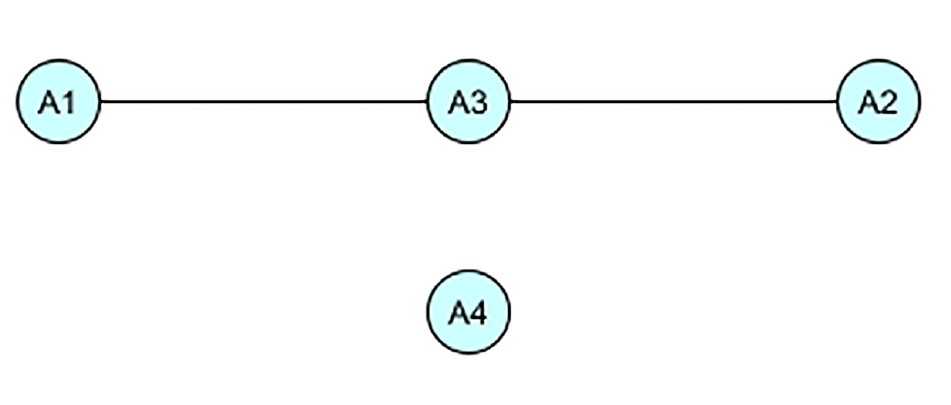
\includegraphics[scale=0.4]{Images/graph_representation.png}
        \end{figure}
        \vspace{-0.5cm}
        %virer
        % \begin{figure}
        %     \centering
        %     \caption{Restriction of the research}
        %      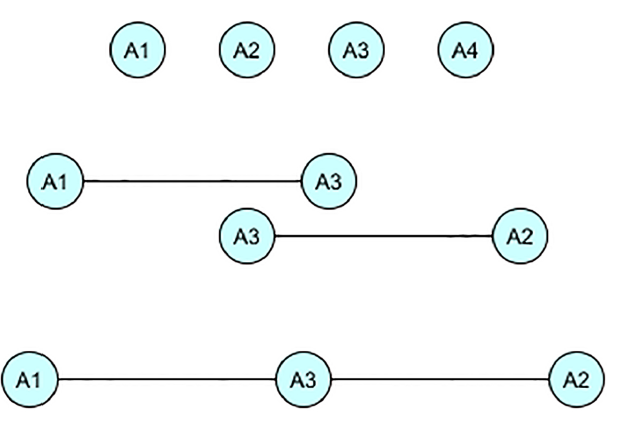
\includegraphics[scale=0.55]{Images/sub_graph.png}
        % \end{figure}
        \justifying
        Remark: The attacker doesn't have such detailed information.
        $\Rightarrow$ The detection of risks is easier for us (the producer) than for him/her (the attacker).
       
    \end{column}
\end{columns}

% \begin{exampleblock}{b-Complexity}
    
% \end{exampleblock}

% \begin{exampleblock}{c-Detection}
    
% \end{exampleblock}
    

  \end{block}

% \vspace{-1cm}

  \begin{block}{2-Protect the cells at risk of overlapping differentiation}

   \begin{columns}
    \begin{column}{0.31\colwidth}
        \vspace{-0.60cm}
        \begin{figure}
            \centering
            \caption{\footnotesize Start}
            \vspace{-1cm}
            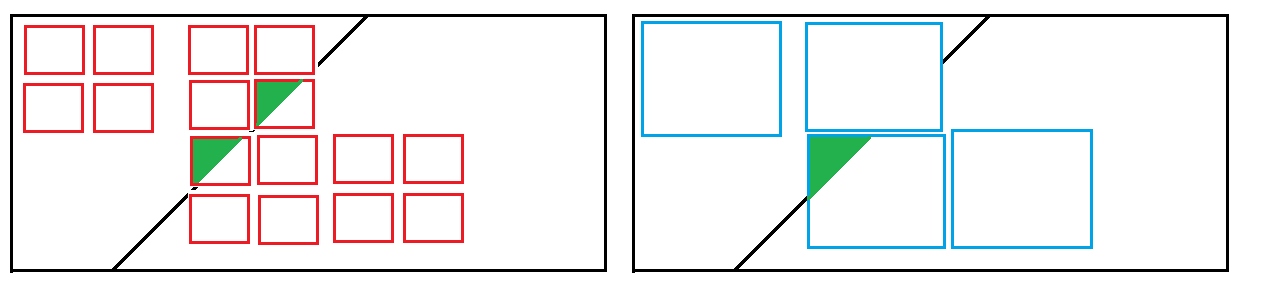
\includegraphics[scale=0.35]{Images/test_articulation.png}
        \end{figure}
        \vspace{-0.5cm}
        \footnotesize
        Legend:
        \begin{itemize}
            \item \colorbox{intersection}{cells}: risky intersections
            \item \colorbox{primary}{cells}: direct protection of the risky intersections
            \item \colorbox{second1}{cells} or \colorbox{second2}{cells}: additional suppression to prepare inter-level diff.
        \end{itemize}
    \end{column}

    \hfill

    \begin{column}{0.31\colwidth}
        \vspace{-1cm}
        \begin{figure}
            \centering
            \caption{\footnotesize Step 1}
            \vspace{-1cm}
            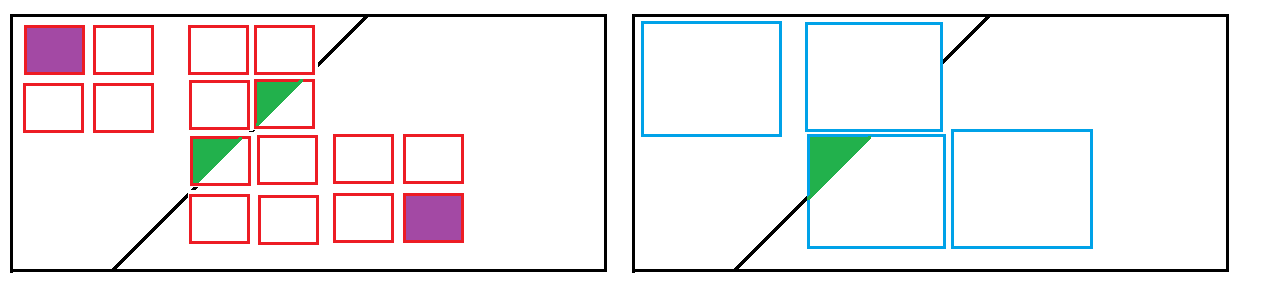
\includegraphics[scale=0.35]{Images/test_articulation_2.png}
        \end{figure}
        \vspace{-1cm}
        \setcounter{figure}{7}
        \begin{figure}
            \centering
            \caption{\footnotesize Step 3}
             \vspace{-1cm}
            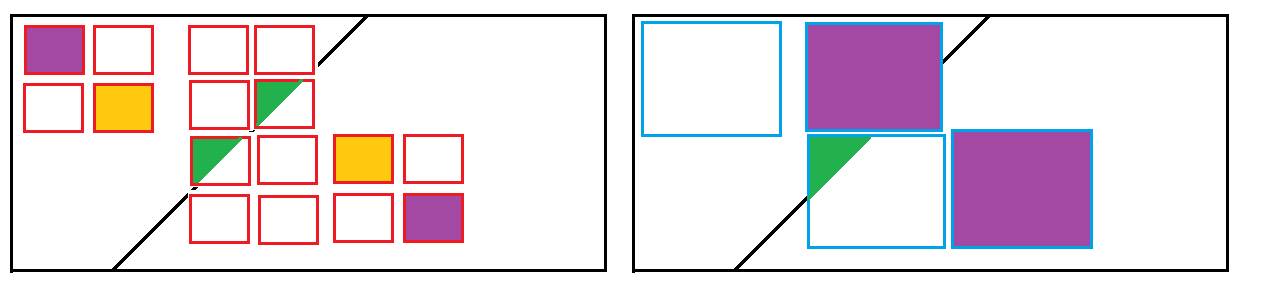
\includegraphics[scale=0.35]{Images/test_articulation_5.png}
        \end{figure}
    \end{column}

    \hfill
    
    \begin{column}{0.31\colwidth}
        
        \vspace{-1cm}
        \setcounter{figure}{6}
        \begin{figure}
            \centering
            \caption{\footnotesize Step 2}
            \vspace{-1cm}
            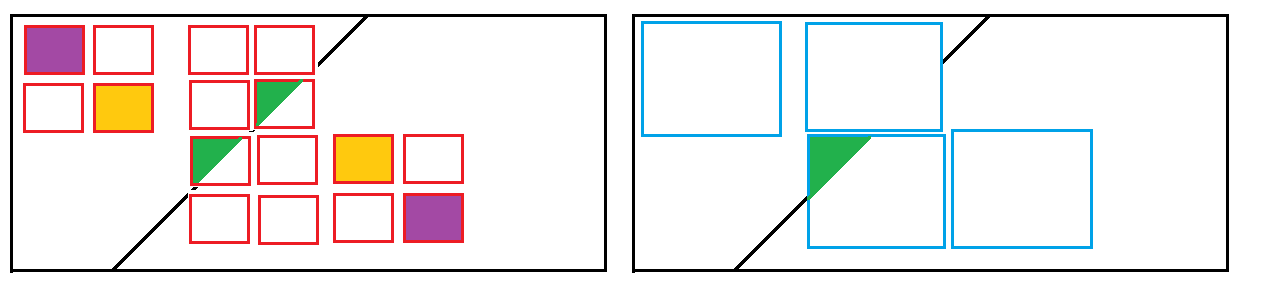
\includegraphics[scale=0.35]{Images/test_articulation_4.png}
        \end{figure}
        \vspace{-1cm}
        \setcounter{figure}{8}
        \begin{figure}
            \centering
            \caption{\footnotesize Step 4}
             \vspace{-1cm}
            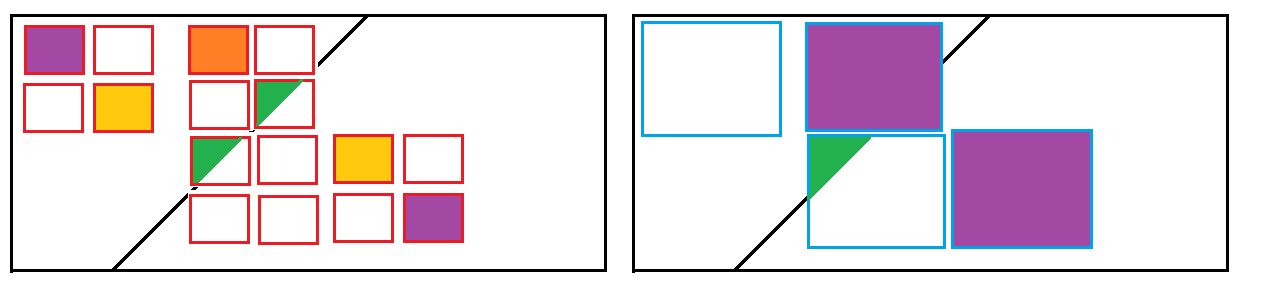
\includegraphics[scale=0.35]{Images/test_articulation_6.png}
        \end{figure}
        
    \end{column}
       
    \end{columns}   

% Legend: In \colorbox{green}{green}, the intersections at risk of differentiation. In \colorbox{purple}{purple}, the cells to "suppress" for a direct protection of the risky intersections. In \colorbox{orange}{orange}, an additional suppression to handle inter-level differentiation.

  \end{block}

% \begin{block}{3-Protect all the risky cells from inter-level differentiation}

    
%     \begin{exampleblock}{a-Idea}

%         The method presented here has been implemented for the fiscal grid data released in 2019 (\cite{gs2018}). It was inspired by the quadtree algorithm. Some adjustments was made to release all the data on the same size of squares. 

%         The idea is to gather risky cells with each other or with some non risky cells to make groups of cells that contain more than the required threshold. The process begins from the coarser level (64km) to the finest one (200m). At each step, the inter-level differentiation is avoided by \textbf{gathering suppressed cells in groups}. These groups are inherited from a level to the next one.

        
%     \end{exampleblock}

% \end{block}

\vspace{1cm}

 \begin{block}{3-Protect all the risky cells from inter-level differentiation}
    \vspace{0.25cm}
    \begin{columns}
        \begin{column}{0.45\colwidth}
            \justifying
            
            The method has been implemented in a \texttt{R} package - optimized in \texttt{C++} - called \texttt{gridy} and applied, the first time, on the fiscal grid data released in 2019 (\cite{gs2018}). It was inspired by the quadtree representation. Some adjustments were made to release all the data on the same size of squares. 
            \newline
            The idea is to gather risky tiles with other ones (and also with some non risky tiles) to make groups that contain more than the required threshold. The process begins from the coarsest level (64km) to the finest one (200m). At each step, the inter-level diff. is avoided by \textbf{gathering suppressed cells in groups}. These groups are inherited from a level to the next one.
            
        \end{column}

        \hfill

        \begin{column}{0.55\colwidth}
            \begin{figure}
                \centering
                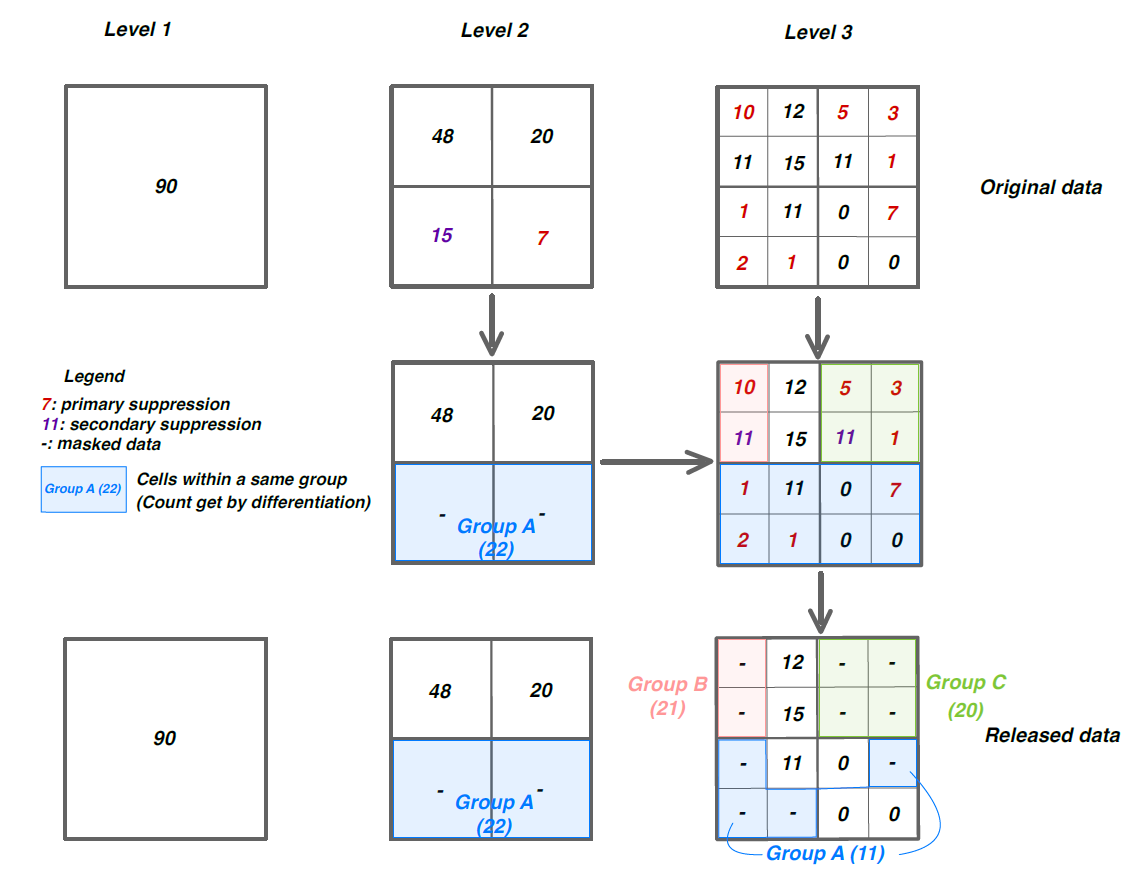
\includegraphics[scale=0.7]{Images/grille_creu_proc_all.png}
                \caption{Handling inter-level diff.}
                \label{fig:my_label}
            \end{figure}
        \end{column}
    \end{columns}

    \vspace{0.5cm}
    \begin{problock}{Which grid levels to use ?}
    To proceed, we need the released grids and at least one another which does not contain any confidential tiles (64km squares grid in France). Using other intermediary grids will generate more secondary suppression while better preserving the spatial structure. For example:
    \begin{itemize}
        \item Using 64km - 1km - 200m levels will generate less cell suppression but perturb more the spatial structure;
        \item Using 64km - 32km - 16km - 8km - 4km - 2km - 1km - 200m levels will generate more cell suppression and perturb less the spatial structure.
    \end{itemize}

    \end{problock}
    
    \end{block}



\end{column}

\separatorcolumn

\begin{column}{\colwidth}
  \vspace{-1cm}
  \begin{block}{4-Protect cells at risk of attributes disclosure}

At this point, we haven't treated the cells at risk of \textit{\textbf{inference disclosure}}. The idea is the following one : once detected, each of these risky cells among the previously non suppressed cells is affected to an existing group of suppressed cells. Two criteria help to choose a good candidate:

\begin{columns}
    \begin{column}{0.48\colwidth}
        \justifying
        \begin{itemize}
        \item \textbf{A distance criterium}: we look for a group not too far from a given risky cell.
    \end{itemize}
    \end{column}
    \hfill    
    \begin{column}{0.48\colwidth}
        \vspace{-0.5cm}
        \begin{itemize}
        \item \textbf{A risk criterium}: we look for a group such that inference won't be possible. 
    \end{itemize}
        
    \end{column}
       
    \end{columns}   

  \end{block}

  \begin{block}{5-Impute data within the groups of suppressed cells}

The suppression process is just temporary: the idea is to release values for each non-empty square. This is the moment \textbf{to use the groups of cells} that have been built during the previous process. The idea is to \textbf{\textit{breakdown the group total}} (for example the number of males) \textbf{\textit{in the tiles of the group, proportionally to the population of each tile}}.

Let $c$ be a tile belonging to a group $g$, with $P^c$ and $P^g$ their respective actual populations, $P^g_m$ and $P^c_m$, their respective actual numbers of males. Then, the imputed counts of males is given by $\hat{p}^c_m &= P^g_m \times \frac{P^c}{P^g}$.

$\Rightarrow$ the totals within each tile are consistent: the sum of the numbers of males and females is equal to the population count.

  \end{block}

  \begin{block}{A limited loss of information}

The protection process is very efficient to minimize the loss of information of the main counts at a fine level (French departments in the figure~\ref{fig:loss}), for breakdown by gender or by age. The loss is more important for small counts as population born abroad.

\begin{figure}
    \centering
    \caption{Differences in \% between the released and the original aggregates by French Department}
    \vspace{-0.5cm}
    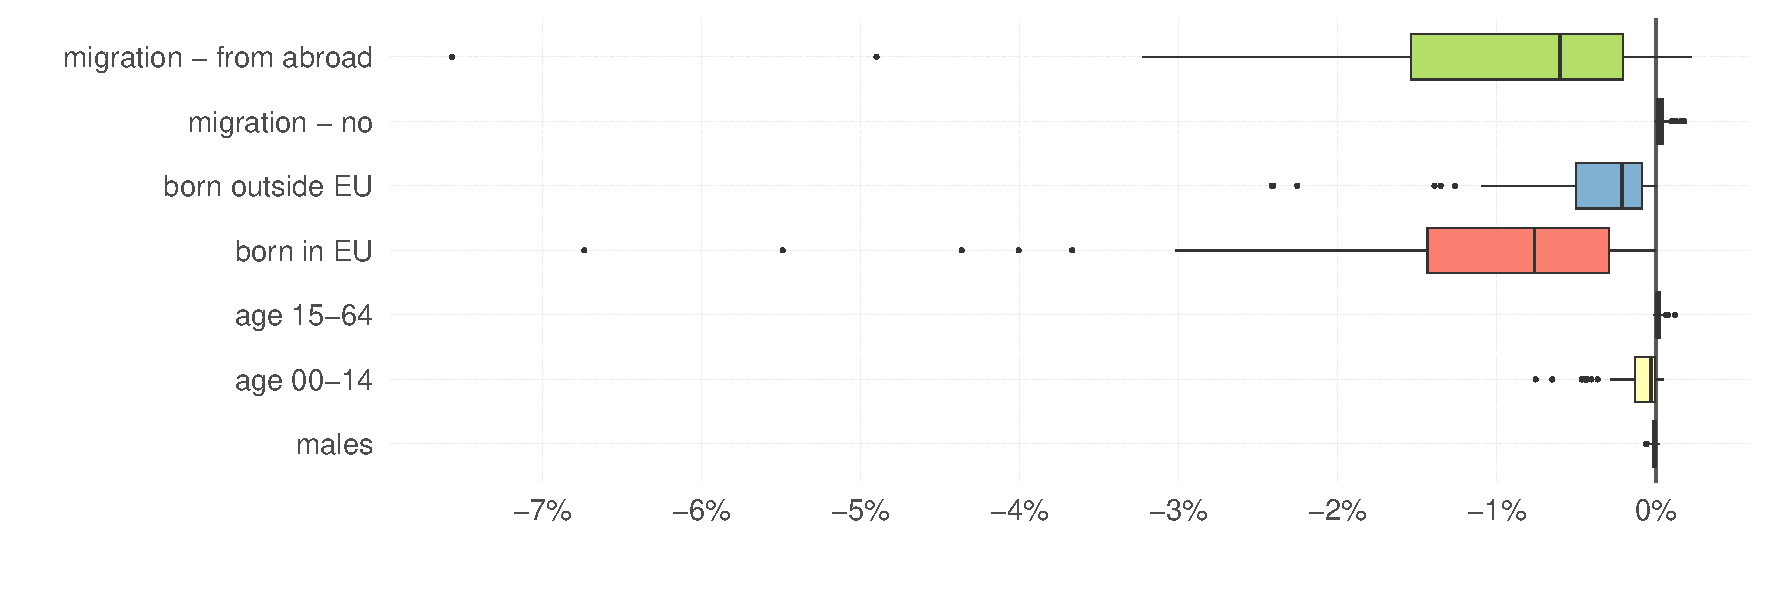
\includegraphics{Images/bilan_departemetal_ecart_pc_pr_poster.pdf}
    \vspace{-1cm}
    \begin{flushleft}
    \footnotesize Note: A department, here, is approximated by all the 1km squares that intersect its effective administrative area.
    \end{flushleft}
    
    \label{fig:loss}
\end{figure}
    
\end{block}  

\vspace{-0.5cm}
  \begin{backblock}{Advantages and Drawbacks}

\underline{\textbf{Advantages}}

\begin{itemize}
    \item A rather general method able to take several confidential issues into account.
    %: attribute disclosure, inference disclosure, inter-level and overlapping differentiations.
    \item The detection of overlapping differentiation is actually very complex for an attacker. With our tool, the complexity level of an attack can be set depending on the scenario of attack which was designed. 
    \item Possibility to monitor the amount of secondary suppression and the perturbation of spatial structures in choosing different levels of grids.
\end{itemize}


\underline{\textbf{Drawbacks}}

\begin{itemize}
    \item Some perturbed cells are not actually perturbed, if an attribute is evenly distributed in every square of a group.
    \begin{itemize}
        % \item If some attributes are evenly distributed in every square of a group, then the perturbation has no effect: $\hat p_c^m = P_g^m \frac{P_c}{P_g} = \beta P_g \frac{P_c}{P_g} = P_c^m$, where $\beta$ is the share of males in each square of the groupe $g$.
        \item As close squares tend to be similar, the hypothesis is a serious one.
        \item But:
        \begin{itemize}
            \item The user doesn't know which cells belong to the same group.
            \item There's no way for the user to know for which cells the hypothesis is really true.
            \item In reality, only the distribution of the gender is really stable among squares. And gender isn't a sensitive attribute.
        \end{itemize}        
    \end{itemize}
    \item The re-identification disclosure risk is not directly handled.
    \begin{itemize}
        \item The original population counts (rounded) are released
        and used to dispatch attributes counts into a group.
        \item But, in our case, the re-identification is only possible with a prior information about the location of a person...
        \item And this re-identification can't lead to obtain much more information on this person.
    \end{itemize}
\end{itemize}
    
  \end{backblock}

\vspace{-2cm}
  \begin{block}{References}

    \nocite{*}
    \scriptsize{\bibliographystyle{plainnat}\bibliography{poster}}

  \end{block}

\end{column}

\separatorcolumn
\end{columns}
\end{frame}

\end{document}

% \begin{figure}
    %   \centering
    %   \begin{tikzpicture}
    %     \begin{axis}[
    %         scale only axis,
    %         no markers,
    %         domain=0:2*pi,
    %         samples=100,
    %         axis lines=center,
    %         axis line style={-},
    %         ticks=none]
    %       \addplot[red] {sin(deg(x))};
    %       \addplot[blue] {cos(deg(x))};
    %     \end{axis}
    %   \end{tikzpicture}
    %   \caption{Another figure caption.}
    % \end{figure}